Sustainable Development Goal 3 (SDG 3), \textit{Good Health and Well-Being} \ref{fig:global_challenges}, aims to improve health outcomes through prevention, early intervention, and access to effective healthcare services. Achieving this goal increasingly depends on the ability of healthcare systems to use available data efficiently and support evidence-based clinical decisions. Data mining and machine learning can contribute to this objective by identifying hidden patterns in routinely collected health information and supporting earlier detection of disease risk.

\begin{figure}[H]
    \centering
    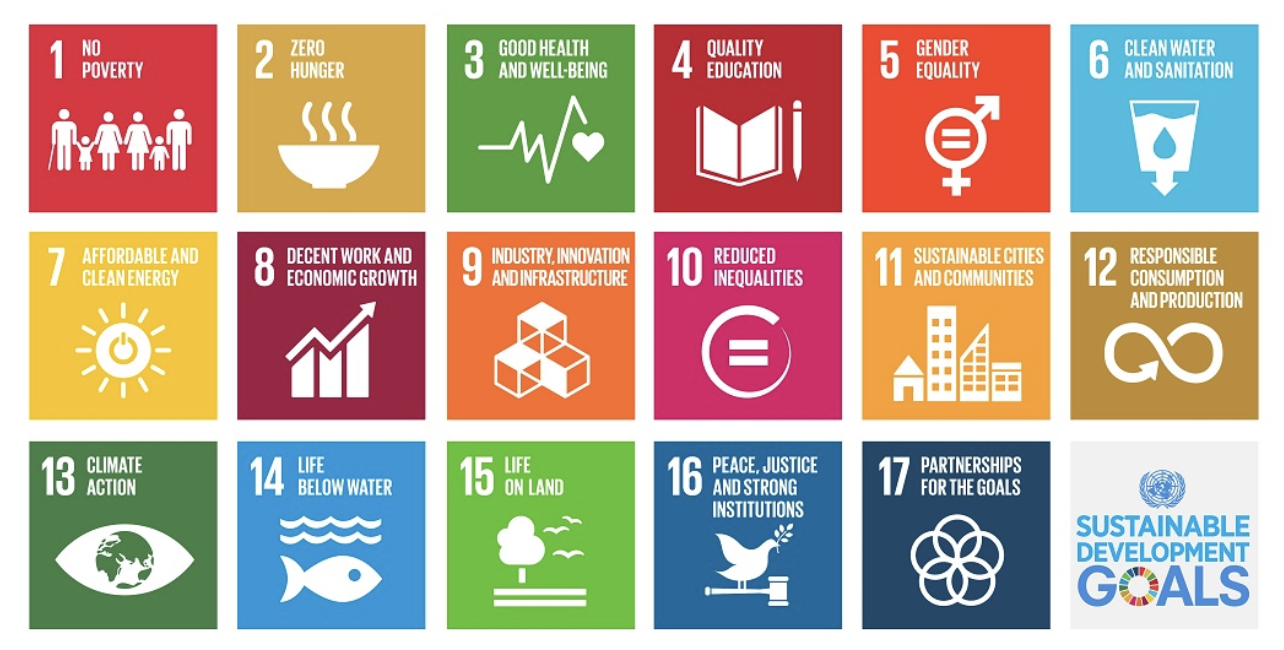
\includegraphics[width=0.8\linewidth]{media/SGD.png}
    \caption{17 Global Challenge for Government Transparency: The Sustainable Development Goals (SDG) 2030 Agenda }
    \label{fig:global_challenges}
\end{figure}

Gallstone disease is a common condition that may remain asymptomatic but can lead to complications such as acute cholecystitis, biliary obstruction, cholangitis, and pancreatitis \parencite{lammert2016gallstones,fujita2023guidelines}. Diagnosis generally relies on clinical assessment and abdominal ultrasonography. However, identifying high-risk individuals before complications occur may support earlier investigation and improve the efficient use of healthcare resources.

This project therefore develops a data-mining solution for the early prediction of gallstone disease using demographic, comorbidity, laboratory, and body-composition information. The Gallstone dataset contains records from 319 participants, including both patients with gallstones and control participants \parencite{esen2024early,uci2025gallstone}. Machine-learning models will be used to identify patterns associated with gallstone status and estimate individual disease risk.

The proposed solution is intended as a clinical decision-support tool rather than a replacement for medical diagnosis. By evaluating predictive performance, sensitivity, interpretability, and important risk factors, the project aims to demonstrate how data-driven healthcare can support preventive intervention, reduce avoidable complications, and improve resource allocation. In this way, the project contributes to a more proactive, efficient, and sustainable healthcare system aligned with the broader objectives of SDG 3.
